\setcounter{page}{1} \pagenumbering{Alph}

% Add PDF bookmark 
\pdfbookmark[0]{Title}{Title}

%%% LOGO
\thispagestyle{empty}
\begin{flushleft} ~\\ \vspace{-12mm} \hspace{-12mm}  
\includegraphics[width=50mm]{Cover/istnewlogo}

    %%% Instituição
    \vspace{5mm}
    \centering
    \Large \textbf{UNIVERSIDADE DE LISBOA \\ INSTITUTO SUPERIOR TÉCNICO}
    %%% espaço sem gráficos
    \vspace{25mm}

    %%% Optional Image
    %\vspace{10mm}
    %~\\ \vspace{50mm} % gráficos
    %\\ \begin{center} 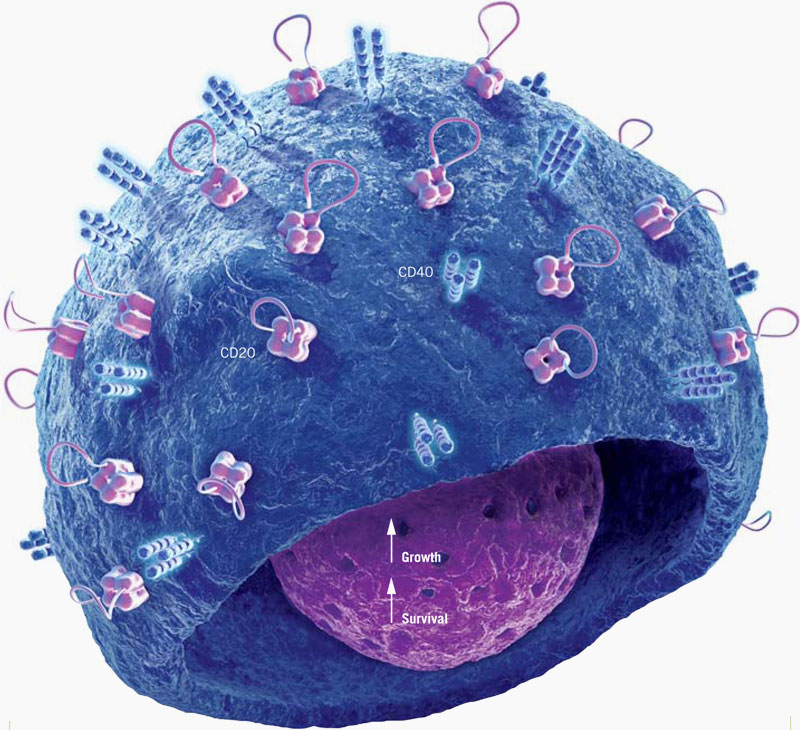
\includegraphics[height=50mm]{Cover/coverimage}  \end{center} % gráficos

    %%% Titulo
    \centering
    \Large \textbf{Learnable Sparsity and Weak Supervision\\for Data-Efficient, Transparent, and Compact Neural Models}
    % \\ \vspace{10mm}
    % \Large Optional Subtitle
    % \\ \vspace{15mm}
    \\ \vspace{25mm}  % NO SUBTITLE
    \large \textbf{Gonçalo Migueis de Matos Afonso Correia} \\
    \vspace{35mm}

    \begin{minipage}{\textwidth}
        \hspace{24mm}
        \begin{tabularx}{\textwidth}{ l @{ } l }
            \centering
            \textbf{Supervisor} :    & Dr. André Filipe Torres Martins \\
            \textbf{Co-Supervisor} : & Dr. Vlad Niculae                \\
        \end{tabularx}
    \end{minipage}
    %
    \\ \vspace{20mm}
    % \vspace{12mm}
    \centering
    \large \textbf{Thesis specifically prepared to obtain the PhD Degree in}\\
    \large Electrical and Computer Engineering\\
    %\\ \vspace{2mm}
    \vspace{18mm}
    \Large \textbf{Draft}

    \vspace{15mm}

    %\large \textbf{\todaythesis\today} \\
    \large \textbf{May 2022} \\
    \let\thepage\relax
\end{flushleft}
\pagebreak
